% Chapter 1

\chapter{Introduction} % Main chapter title

\label{Chapter1} % For referencing the chapter elsewhere, use \ref{Chapter1} 

%----------------------------------------------------------------------------------------

% Define some commands to keep the formatting separated from the content 
\newcommand{\keyword}[1]{\textbf{#1}}
\newcommand{\tabhead}[1]{\textbf{#1}}
\newcommand{\code}[1]{\texttt{#1}}
\newcommand{\file}[1]{\texttt{\bfseries#1}}
\newcommand{\option}[1]{\texttt{\itshape#1}}

%----------------------------------------------------------------------------------------

\section{Parental controls}

\subsection{Overview}
Parental controls \cite{parentalControls} are the names for a group of settings that gives control to the parent of the content the children can see online. It developed in the digital era as a means to allow parents to restrict the access of content to their children and may be included in digital television services, computer and video games and mobile devices. More than 90\% of parents  of 5-15s who use parental control software consider it useful. \citep{ofcom2017children} The content may not be appropriate for their age and is aimed more at adult audiences. The characteristics of inappropriate content depends for each parent, and is also correlated with the child's age and maturity level and includes information and images that can upset the child, inaccurate information or information that can cause dangerous behavior. Such content can be classified in the following categories:

\begin{itemize}
\item pornographic material
\item content containing swearing
\item sites that encourage vandalism
\item pictures, videos or games which shows images of violence
\item gambling sites
\item unmoderated chatrooms
\end{itemize}

It is very easy for the child to stumble upon unsuitable sites by accident on any Internet enabled device, like mobile phone or tablet and it can be difficult to monitor and filter the content. \parencite{innapropriateContent}

Parental control solutions fall into four categories:

\begin{itemize}
\item content filters, which limit access to different types of inappropriate content
\item usage control, which works by constraining the usage of certain devices by placing time-limits on usage or forbid some types of usage
\item computer usage management tools, which enforces the use of certain software
\item monitoring, which can track the activity when using the devices
\end{itemize}

The rising availability of the Internet increased the demand for methods of parental control that restrict content. Mobile phones offer the most convenient and constant method for content access, and teens ages 13 to 17 are going online frequently. A study by Pew Research Center found that 92\% of teens report going online daily, 24\% of which are using the Internet almost constantly, 56\% going online several times a day and 12\% reporting once a day use. Only 6\% go online weekly and 2\% less often. \parencite{lenhart2015teens}

\begin{figure}[th]
\centering
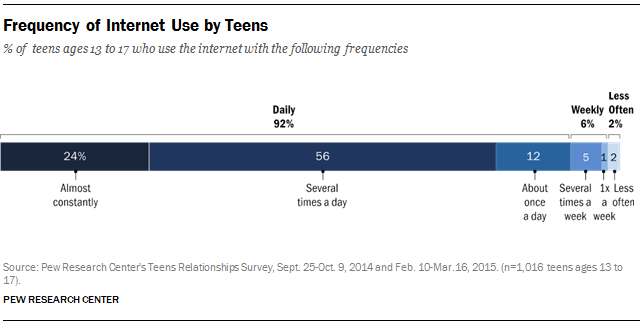
\includegraphics[width=1\textwidth]{Figures/frequency-of-internet-use-by-teens}
\decoRule
\caption[Frequency of Internet Use by Teens]{Frequency of Internet Use by Teens}
\label{fig:frequency-of-internet-use-by-teens}
\end{figure}

The same study finds that nearly three-quarters own or have access to a smartphone and only 30\% have a basic phone and 12\% of teens, 13 to 17, have no cell phone of any type.

\subsection{Techniques}

There are two types of control techniques:
\begin{itemize}
\item behavioral control, which consists of controlling the amount of time and how much the child can consume;
\item psychological control, which involves parents tying to influence children by affecting their emotional side by manipulating or insensitivity;
\end{itemize} 

Adult control can be divided into three prototypes, each of which has influenced greatly the child-rearing practices \parencite{baumrind1966effects}:

\begin{itemize}
\item permissive: the parent attempts to behave in a nonpunitive, acceptant and affirmative manner and consult with the child about policy decisions and gives explanations for rules
\item authoritarian: the parent attempts to shape, control and evaluate the behavior of the child in accordance with a set standard of conduct, by valuing obedience as a virtue and favoring punitive, forceful measures to curb self-will
\item authoritative: the parent attempts to direct the child's activities in a rational manner, by sharing the reasoning behind the policy and soliciting the child's objections when he refuses to conform; disciplined conformity and autonomous self-will are valued by the authoritative parent
\end{itemize}

Several techniques exists for creating parental controls to block certain websites. Parental control software can monitor API to observe applications such as web browsers or chat applications and to intervene based on certain criteria, such as time based criteria or as a match in a database of banned words. Other techniques that involve a proxy server are also used, in which the proxy server serves as an intermediary. The proxy server can use content based filters to intervene in the delivery of some content, but this method has a major disadvantage because it requires client configuration to use the service, which can be easily bypassed.

The difference between content filters and computer usage management methods is that the later is focused on empowering the parents to balance the computing environment for children. It does so by allowing parents to enforce the learning component into the computing time of children, where children can earn play time by working through educational content. This method is very powerful because it stimulates self-regulation in children, instead on relying solely on parental control, and we will use some ideas from this method to develop our control and regulation system.

Recently, some devices which are used for network based parental control have emerged. These devices use different methods to block inappropriate content, such as packet filtering, DNS Response Policy Zone (RPZ) and Deep packet inspection (DPI) \citep{vixie2010dns}, and work as a firewall router. Some commercial and governmental communication networks use these methods also, but these type of devices were developed for home also, and are used to create a new home wireless network specifically designed for kids to connect to. We developed our system using the same approach, by creating a custom wireless network for different type of users, different age level children and parents, and by using the packet filtering and DNS techniques to manage content filters.

\subsection{Content filters}

The increased use of mobile devices has created a demand for parental controls for these devices. The first carrier which offered age-appropriate content filters was Verizon, in 2007. With the release of iPhone OS 3.0 in 2009, Apple introduced a mechanism to create age brackets for users, to block unwanted applications from being downloaded. Filtering options are also offered by most Internet providers, to limit Internet browsing options and block unsuitable content. The software used to restrict or control the content a user is capable to access is commonly referred to as Internet filter or content filter.

The content access restrictions can be applied at different levels, from governments applying them nationwide, to ISP blocking it's clients and by a parent to a child's computer. The content filtering mechanism can be implemented at different levels also, either by software on the client computer or by using the network infrastructure such as proxy servers, DNS servers and firewalls, but a mix of these technologies provides the most complete content control coverage.

\begin{itemize}
\item Browser based filters are the most lightweight solution, and the filtering is done by using a third-party browser extension
\item E-mail filters are commonly implemented using a statistical method, Bayesian filters \citep{sahami1998bayesian}, by acting on information contained in the mail body, headers or attachments
\item Client side filters work by installing it as software on each target device
\item Content-limited (or filtered) ISPs are service providers that offer access to only a set of Internet content, to implement government, regulatory or parental control over its subscribers
\item Network-based filtering is done at the transport layer, by implementing a transparent proxy, redirecting user requests to it by a switch or a router, or at the application layer, by configuring the client to send requests directly to the proxy server. \parencite{contentGateway}
\item DNS-based filtering \citep{sarvepalli2017dns} is implemented at the DNS layer and works by preventing lookups for domains that do not fit within a set of rules, parental control or company rules
\item Search-engine filters work by filtering out inappropriate search results, but if the client knows the URL for a specific content, he can access it without using a search engine; search providers offers child friendly versions of their engines, which filter content inappropriate for children from the search results
\end{itemize}

We implement a DNS-based filtering mechanism, to be able to easily filter out the content that is definitely harmful for a child and does not bring any value, while not being too restrictive and giving the children room to explore and find by themselves what values means and how the time is best spent on the device. The main reason for filtering is to protect the user from harmful content, but it is used also to block malware and other intrusive material, as adware, spam, computer viruses, spyware, which can be even more harmful to children. The first level of filtering that we try to do is to block ads by integrating with the open-source ad-blocking solution Pi-hole \citep{pot2015adblock}, which works as a DNS sinkhole to block advertisement and Internet trackers.

Filtering mechanisms are not always efficient, and are also subject to some criticism. The filtering errors are of two kinds, overblocking, when the filter is too zealous and mislabels content that should be acceptable, such as labeling health related information as being porn-related, because of the Scunthorpe problem \citep{anh2015scunthorpe}, and under-blocking, when the filter is unable to update quickly to new information available on the Internet. Content filtering can be a powerful censorship tool and there is a lot of discussion around the morality and legality of this kind of methods at a certain level, mostly state and country level. But it can be harmful if used incorrectly even at the family level, because using too strict policies can influence children behavior, and not always for good.

%----------------------------------------------------------------------------------------

\section{A self regulation approach}

An in-depth study conducted on 75 Android apps that have the main purpose of promoting teens and children mobile online safety found that the majority of them (89\%) are supported by features of parental control, and only 11\% favour self-regulation. \citep{wisniewski2017parental} The study presented a framework for Teen Online Safety Strategies which describes the difference between parental control and teen-self regulation. The three main parental control strategies identified are:

\begin{itemize}
\item monitoring is the surveillance of online activities, such as text messages, call logs or web browser history; Some studies found that monitoring was associated with higher online risks for some, suggesting to use monitoring only after some kind of online problem occurred.\parencite{duerager2012can}
\item restriction occurs by placing rules on online activities, as setting limits on screen time and content acceptable for viewing. This kind of methods have some positive impact, such as reducing cyberbullying, but can also have negative effects, by causing children to take more risk-seeking behaviors. \parencite{shin2014exploring}
\item active mediation involves discussions regarding online activities between parents and children, and it reduces online risks without reducing the benefits of online engagement. \parencite{duerager2012can}
\end{itemize}

Self-regulation is the ability to control the emotions and behaviors by monitoring and evaluating oneself against given social standards. The analogous teen self-regulation strategies are:

\begin{itemize}
\item self-monitoring is a key component of self-regulation, and children must be aware of their own motivations and actions through self-observation. \parencite{bandura1991social}
\item impulse control is the ability to inhibit short term desires in favor of the long term consequences caused by ones' actions, and losing control of this is the main reasons why self-regulation fails \parencite{baumeister1996self}
\item risk-coping is a self-regulatory process that occurs after a stressful situation, by attempting to address the problem and the negative emotions caused. Actively coping with risky online situations help teens to feel less bothered about a risky event that occurred. \parencite{d2013cope}
\end{itemize}

Usability was another issue in finding a good and efficient parental control mobile application. From the 89 application tested, 14 had configuration issues, some required users to have a Gmail account, other needed a VPN connection configured, some where showing annoying ads. Other apps were not meeting the goal of protecting the children from online risks, most of them were focusing on regulating web browsing and social media was one of the least prevalent activity monitored, but research suggest that most online risks, at least for adolescents, are encountered through the use of social media platforms. The features offered did not promote any values like trust, accountability, respect and transparency.

Most of the apps related to parental controls support mostly monitoring and restriction of mobile activities. Only some of the them support features like parental active mediation (<1\%), teen risk-coping (4\%), self monitoring (2\%), or impulse control (<1\%), but some of them added education as another safety strategy. We will try to have a different approach, by focusing more on the self-regulation approach while keeping the monitoring and restriction features to the minimum necessary, and try to add the education component also, to drive children to some learning resources and interactive quizes before rewarding them with some device time.

We try to design our solution by following the practices suggested in the study from \parencite{wisniewski2017parental} and to focus on usability, social media control and to implement features that match the self regulation techniques. To be able to have more granular control and to implement specific features for each age, we create 4 age brackets, 0-5, 6-10, 11-13, and 14+. We try to design the application to be used mostly as a tool of communication between the children and the parents, not just a tool for enforcing the parents rules, by encouraging discussion about the rules being set. The process of establishing the rules and starting the parental control system should be done also as a collaboration between parents and children. The current solutions are fairly simplistic: as new functionality becomes available, new apps are created to regulate and monitor the children activities. While these approach prevent the risks, it also has the potential of limiting some positive engagement. As we can see in figure \ref{fig:current-vs-proposed}, the new framework proposed for developing mobile online safety application is founded on core family values and emphasizes parental active mediation and self-regulation. The benefit of this framework is that it is not technically tied directly to children mobile activities and can focus on supporting more important needs of parents and children. We propose prototypes to promote collaborative practices between parents and children that support risk-coping and active parental mediation, by implementing a system for the children to learn about online risks and encouraging collaborative efforts when establishing policies. Another unique opportunity for design is in the are of supporting self-regulatory processes in the absence of parents. Instead of simply giving an SOS feature to get help from adults, some other ways to support the children can be found, so that they can come up with their solutions to online problems or to come to the aid of others who could benefit from their help.

\begin{figure}[th]
\centering
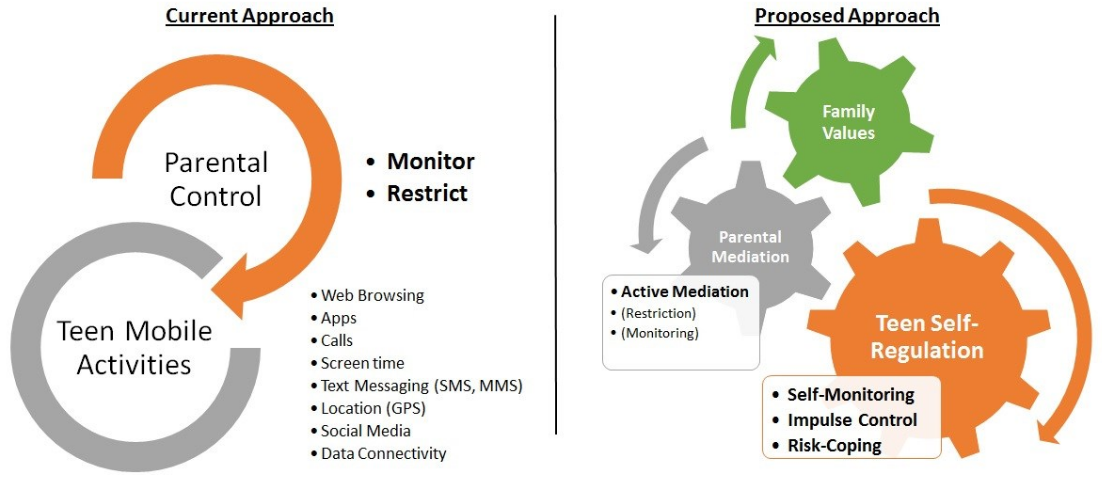
\includegraphics[width=1\textwidth]{Figures/current-vs-proposed}
\decoRule
\caption{Current versus Proposed Approach for Online Safety Apps}
\label{fig:current-vs-proposed}
\end{figure}

%----------------------------------------------------------------------------------------
